\documentclass[10pt,fleqn]{beamer}

\usepackage{graphicx}
\usepackage{amsmath,amssymb}
\usepackage{bm}
\usepackage{zxjatype}
\usepackage[ipa]{zxjafont}
\usepackage{tikz}
\usepackage{tikzsymbols}

\usetikzlibrary{backgrounds,positioning}
\usetheme[progressbar=frametitle]{metropolis}
\usefonttheme[onlymath]{serif}

\DeclareMathOperator*{\argmax}{argmax}

\newcommand{\myinsertlogo}[1]{%
\begin{tikzpicture}[overlay, remember picture]
    \node[above left=1cm and .8cm of current page.south east] {\includegraphics[width=2.25cm]{#1}};
\end{tikzpicture}}

\title{{\large ディリクレ過程混合モデルによるクラスタリング}}
\subtitle{続・わかりやすいパターン認識 第12章}
\date{October 8, 2018}
\author{Satoshi Murashige}
\institute{Mathematical Informatics Lab., NAIST}

\begin{document}
    \begin{frame}{}
        \maketitle
        \myinsertlogo{naist.pdf}
    \end{frame}
    \begin{frame}{Title}
        Hello metropolis!
    \end{frame}
    \begin{frame}{Table of Contents}
        \tableofcontents
    \end{frame}
    \begin{frame}{モチベーション:\\ クラスタ数が未知のクラスタリング問題を解きたい}
        \begin{center}
            \includegraphics[width=10cm]{scatter.pdf}
        \end{center}
    \end{frame}
    \begin{frame}{生成モデル:観測パターンの生成過程をモデル化する}
        \begin{tikzpicture}
            \tikzstyle{model node}=[draw, inner sep=0pt, outer sep=0pt, node distance=2.5cm]
            
            \node[] (cluster) {
                \begin{tikzpicture}
                    \draw (0, 0) -- (2.5, 0);
                    \draw (0.3, 0.0) coordinate (a1) -- ++(0, 1.5);
                    \draw (0.6, 0.0) coordinate (a2) -- ++(0, 1);
                    \draw (0.9, 0.0) coordinate (a3) -- ++(0, 1.2);
                    \draw (1.2, 0.0) coordinate (a4) -- ++(0, 0.8);
                    \draw (1.5, 0.0) coordinate (a5) -- ++(0, 0.4);
                    \node[anchor=north] at (a1) {1};
                    \node[anchor=north] at (a2) {2};
                    \node[anchor=north] at (a3) {3};
                    \node[anchor=north] at (a4) {4};
                    \node[anchor=north] (n5) at (a5) {5};
                    \node[anchor=west] at (n5.east) {$\cdots$};
                \end{tikzpicture}
            };
            
            \node[model node, right of=cluster, node distance=4.5cm] (gauss2) {\includegraphics[width=3cm]{gauss2.pdf}};
            \node[model node, above of=gauss2, node distance=2.6cm] (gauss1) {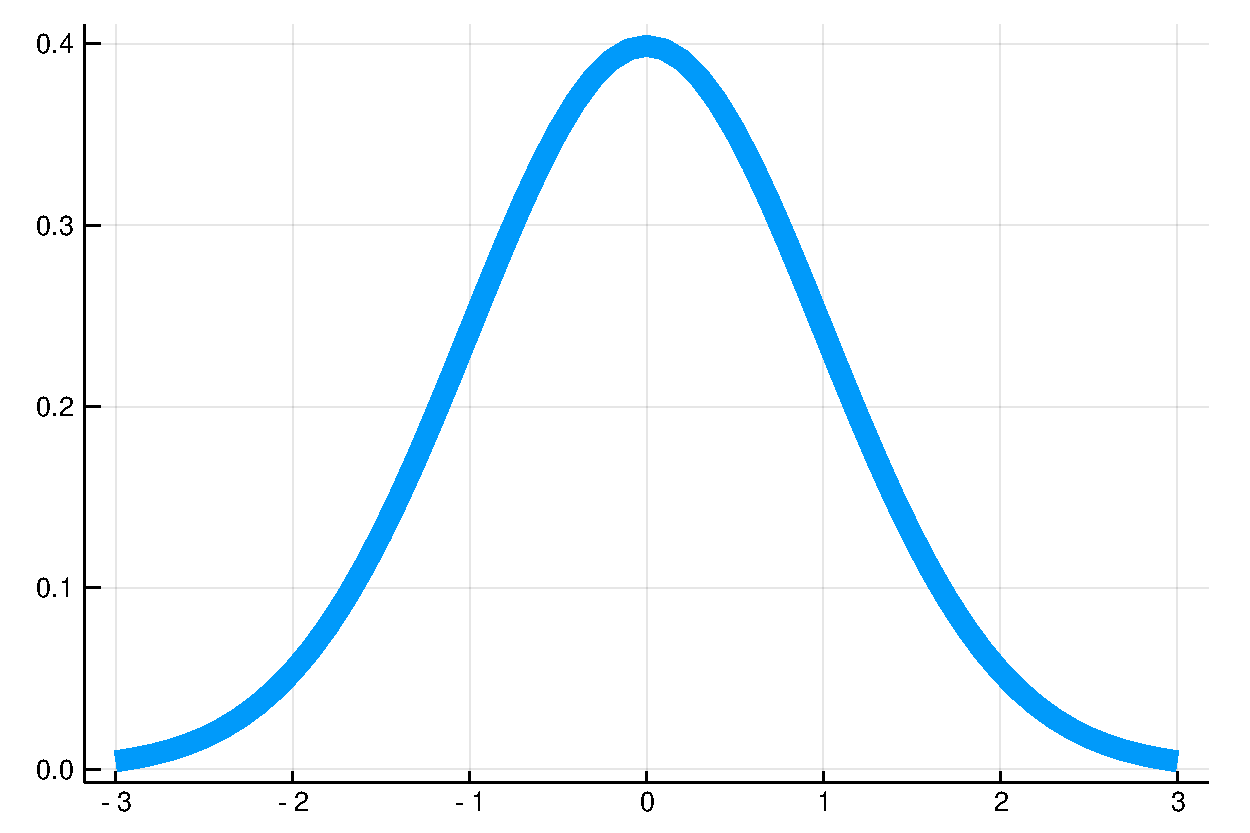
\includegraphics[width=3cm]{gauss1.pdf}};
            \node[model node, below of=gauss2, node distance=2.6cm] (gauss3) {\includegraphics[width=3cm]{gauss3.pdf}};
            
            \node[anchor=south] at (gauss1.north) {クラスタ1: $\bm\theta_1 = (\bm\mu_1, \Sigma_1)$};
            \node[anchor=south] at (gauss2.north) {クラスタ2: $\bm\theta_2 = (\bm\mu_2, \Sigma_2)$};
            \node[anchor=south] at (gauss3.north) {クラスタ3: $\bm\theta_3 = (\bm\mu_3, \Sigma_3)$};
            
            \node[anchor=south] at (cluster.north) {$s_n\sim\mathrm{Categorical}(s|\bm\pi)$};
            
            \node[right of=gauss1, node distance=4.0cm, scale=2.0] (x1) {$\mathbf x_1$};
            \node[below of=x1, node distance=1.0cm, scale=2.0] (x2) {$\mathbf x_2$};
            \node[below of=x2, node distance=1.0cm, scale=2.0] (x3) {$\mathbf x_3$};
            \node[below of=x3, node distance=1.0cm, scale=2.0] (x4) {$\mathbf x_4$};
            \node[below of=x4, node distance=1.0cm, scale=2.0] (x5) {$\mathbf x_5$};
            
            \node[anchor=south] at (x1.north) {$\mathbf x_n \sim \mathcal N(\mathbf x|\bm\mu_c, \Sigma_c)$};
            
            \tikzstyle{cluster arrow}=[-latex, dashed, line width=1pt]
            \draw[cluster arrow] (cluster.east) to[] (gauss1.west);
            \draw[cluster arrow] (cluster.east) to[] (gauss2.west);
            \draw[cluster arrow] (cluster.east) to[] (gauss3.west);
            
            
            \tikzstyle{generate arrow}=[-latex, line width=1pt]
            
            \draw[generate arrow] (gauss1.east) to[bend left] (x1.west);
            \draw[generate arrow] (gauss1.east) to[bend left] (x3.west);
            \draw[generate arrow] (gauss2.east) to[bend left] (x4.west);
            \draw[generate arrow] (gauss3.east) to[] (x2.west);
            \draw[generate arrow] (gauss3.east) to[bend right] (x5.west);
            
            \node[anchor=north] at (gauss3.south) {$\vdots$};
            \node[anchor=north] at (x5.south) {$\vdots$};
            
        \end{tikzpicture}
    \end{frame}
    \begin{frame}{観測パターンの生成過程のグラフィカルモデル}
        \begin{center}
            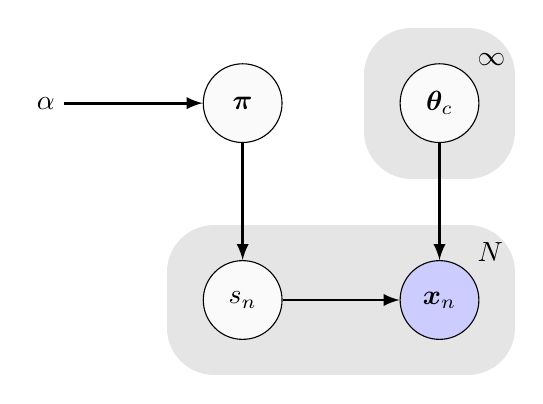
\begin{tikzpicture}
                \tikzstyle{latent}=[draw, circle, minimum size=1cm, node distance=2.5cm, fill=black!2]
                \tikzstyle{observed}=[latent, fill=blue!20]
                \tikzstyle{edge}=[-latex, line width=1pt]
                
                \node[] (a) {$\alpha$};
                \node[latent, right of=a] (pi) {$\bm\pi$};
                \node[latent, below of=pi] (s) {$s_n$};
                \node[observed, right of=s] (x) {$\bm x_n$};
                \node[latent, above of=x] (t) {$\bm \theta_c$};
                
                \draw[edge] (a) -- (pi);
                \draw[edge] (pi) -- (s);
                \draw[edge] (s) -- (x);
                \draw[edge] (t) -- (x);
                
                \node[anchor=south west] at (t.north east) {$\infty$};
                \node[anchor=south west] at (x.north east) {$N$};
                
                \begin{pgfonlayer}{background}
                    \filldraw[line width=12mm, join=round, black!10] (s.north west) rectangle (x.south east);
                    \filldraw[line width=12mm, join=round, black!10] (t.north west) rectangle (t.south east);
                \end{pgfonlayer}
            \end{tikzpicture}
        \end{center}
    \end{frame}
    \begin{frame}{クラスタリング問題の定式化}
        \begin{align*}
            p(\mathbf s, \bm\theta | \mathbf x)
            &= \frac{p(\mathbf x, \mathbf s, \bm\theta)}{p(\mathbf x)}
            = \frac{p(\mathbf x | \mathbf s, \bm\theta)P(\mathbf s)p(\bm\theta)}{\displaystyle \sum_{\mathbf s}\int p(\mathbf x | \mathbf s, \bm\theta)P(\mathbf s)p(\bm\theta)d\bm\theta} \tag{11.4}\\
            (\hat{\mathbf s}, \hat{\bm\theta}) &= \argmax_{\mathbf s,\bm\theta}\left\{ p(\mathbf s, \bm\theta | \mathbf x) \right\} \tag{11.5}
        \end{align*}
        \begin{enumerate}
            \item 事前確率$P(\mathbf s)$をどのように決めるか?
                \begin{itemize}
                    \item クラスタ数が無限にあるので,工夫が必要
                \end{itemize}
            \item 事後確率$p(\mathbf s, \bm\theta | \mathbf x)$をどのように最大化するか?
                \begin{itemize}
                    \item $\mathbf s$のあらゆる組合せを考えるのは不可能
                \end{itemize}
        \end{enumerate}
    \end{frame}
    
    \begin{frame}{事前確率$P(\mathbf s)$はデータをクラスタに分割する方法の確率モデル}
        \begin{center}
            \begin{tabular}{c|c}\hline 
                 クラスタリング&CRP \\ \hline 
                 $k$個目のパターン$\mathbf x_k$ & $k$人目の客 \\
                 総パターン数$n$ & 来店客数 \\
                 クラスタ$\omega_i$ & テーブル$i$ \\
                 クラスタ数$c$ & 使用するテーブル数 \\
                 クラスタ$\omega_i$のパターン数$n_i$ & テーブル$i$に座った人の数 \\ \hline 
            \end{tabular}
        \end{center}
    \end{frame}
    
    \begin{frame}{クラスタ数未知のクラスタリング問題におけるデータの生成過程の定式化}
        \begin{align*}
            &s_1,\cdots,s_n | \alpha \sim \mathrm{CRP}(\alpha) \tag{12.4}\\
            &\bm\theta_i | \beta \sim G_0(\bm\theta) \tag{12.5}\\
            &\mathbf x_k | s_k = \omega_i,\theta \sim p(\mathbf x | \bm\theta_i) \tag{12.6} 
        \end{align*}
    \end{frame}
    
    \begin{frame}{事後確率$p(\mathbf s, \bm\theta | \mathbf x)$の最大化問題を解きたい}
        \begin{align*}
            (\hat{\mathbf s}, \hat{\bm\theta}) &= \argmax_{\mathbf s,\bm\theta}\left\{ p(\mathbf s, \bm\theta | \mathbf x) \right\} \tag{11.5}
        \end{align*}
        \begin{alertblock}{アプローチ}
            \begin{itemize}
                \item あらゆる組合せの$\mathbf s$を評価するのではなく,
                    ランダムサンプリングした$\mathbf s$の中から$p(\mathbf s, \bm\theta | \mathbf x)$を最大化するものを選ぶ
                \item ランダムサンプリングにはGibbsサンプリングを用いる
            \end{itemize}
        \end{alertblock}
    \end{frame}
    
    \begin{frame}{Second Frame}
        \begin{align}
            &G(\bm \theta) | \alpha, G_0(\bm \theta) \sim \mathrm{DP}(\alpha, G_0(\bm \theta)) \tag{12.1}\\
            &\bm \theta^k  \sim G(\bm \theta) & (k = 1,\cdots,n) \tag{12.2}\\
            &\mathbf x_k|\bm\theta \sim p(\mathbf x|\bm \theta^k) & (k = 1,\cdots,n) \tag{12.3}
        \end{align}
    \end{frame}
    \section{12.1 ディリクレ過程混合モデルとその学習法}
    \subsection{[1] クラスタリング法1:所属クラスタとそのパラメータの決定}
    \subsection{[2] クラスタリング法2:所属クラスタのみ決定}
    \section{12.2 ノンパラメトリックベイズモデルの実験}
    \subsection{[1] クラスタリング法1の実験}
    \subsection{[2] クラスタリング法2の実験}
    \begin{frame}{データの生成過程の具体例:ニュース記事の生成過程}
        \begin{align}
            &G(\bm \theta) | \alpha, G_0(\bm \theta) \sim \mathrm{DP}(\alpha, G_0(\bm \theta)) \tag{12.1}\\
            &\bm \theta^k  \sim G(\bm \theta) & (k = 1,\cdots,n) \tag{12.2}\\
            &\mathbf x_k|\bm\theta \sim p(\mathbf x|\bm \theta^k) & (k = 1,\cdots,n) \tag{12.3}
        \end{align}
    \end{frame}
    \begin{frame}{Dirichlet過程混合モデルによるデータの生成過程の記述}
        \begin{align}
            &G(\bm \theta) | \alpha, G_0(\bm \theta) \sim \mathrm{DP}(\alpha, G_0(\bm \theta)) \tag{12.1}\\
            &\bm \theta^k  \sim G(\bm \theta) & (k = 1,\cdots,n) \tag{12.2}\\
            &\mathbf x_k|\bm\theta \sim p(\mathbf x|\bm \theta^k) & (k = 1,\cdots,n) \tag{12.3}
        \end{align}
    \end{frame}
    \begin{frame}{Remark: Chinese Restaurant Process(CRP) は客がテーブルを選択する過程をモデル化したもの}
        \begin{align}
            &s_1,\cdots s_n| \alpha \sim \mathrm{CRP}(\alpha) \tag{12.4}\\
            &\bm \theta_i | \beta \sim G_0(\bm \theta) & (i = 1,\cdots,\infty) \tag{12.5}\\
            &\mathbf x_k|s_k = \omega_i,\bm\theta \sim p(\mathbf x|\bm \theta_i) & (k = 1,\cdots,n) \tag{12.6}
        \end{align}
        \begin{itemize}
            \item CRPでは,無限個のテーブルがある料理店を考えているので,クラスタの数が無限にある.
            \item $\alpha$ は新しいテーブルが選ばれる確率
        \end{itemize}
    \end{frame}
    \begin{frame}{生成モデルの学習:観測パターンからモデルの潜在変数やパラメタの事後分布を推定する}
        \begin{itemize}
            \item CRP
        \end{itemize}
    \end{frame}
    \begin{frame}{生成モデルによるクラスタリングのモデル化とGibbsサンプリングによる学習}
        \begin{itemize}
            \item CRP
        \end{itemize}
    \end{frame}
    \begin{frame}{Bayes推定に基づくクラスタリングのモデル化:\\ クラスタ割当てとクラスタのモデルパラメタが未知}
        \begin{itemize}
            \item クラスタリング問題の確率モデルを立てる
            \begin{align*}
                \mbox{\scriptsize パターン:}
                &\mathbf x = \{\mathbf x_1, \cdots, \mathbf x_n\}  \tag{11.1}\\
                \mbox{\scriptsize パターンのクラスタ割当て:}
                &\mathbf s = \{s_1, \cdots, s_n\} \tag{11.2}\\
                \mbox{\scriptsize 各クラスタのモデルパラメタ:}
                &\bm \theta  = \{\bm \theta_1, \cdots, \bm \theta_c\}   \tag{11.3}
            \end{align*}
            \item Bayesの定理から事後確率を計算する
            \begin{align}
                p(\mathbf s, \bm \theta|\mathbf x)
                = \frac{p(\mathbf x|\mathbf s,\bm\theta)P(\mathbf s)p(\bm\theta)}{p(\mathbf x)}
                = \frac{p(\mathbf x|\mathbf s,\bm\theta)P(\mathbf s)p(\bm\theta)}{\sum_{\mathbf s}{\displaystyle\int p(\mathbf x|\mathbf s,\bm\theta)P(\mathbf s)p(\bm\theta)d\bm\theta}} \tag{11.4}
            \end{align}
            \item 事後確率最大化によりクラスタ割当て・パラメタを決定
            \begin{align*}
                (\hat{\mathbf s}, \hat{\bm \theta})
                = \argmax_{\mathbf s,\bm\theta}\left\{ P(\mathbf s,\bm\theta|\mathbf x) \right\}\tag{11.5}
            \end{align*}
        \end{itemize}
    \end{frame}
\end{document}